\subsection{A certified controller with hidden, action-dependent liquidity}
\label{sec:partialexperiment}

This experiment implements \cref{thm:computablepartial,prop:partialmeshrate,cor:partialsignature}.
The controller does not observe the liquidity regime,
and its actions change the future regime and its reports. Every optimality
bound below is a finite-model calculation. The model is synthetic, with no
calibration or claim about realized exchange performance.

\subsubsection*{Model, information and feasibility}

The parent is 1,000 shares, represented by $q_0=10$ units of 100 shares,
with $K=12$ decisions. Hidden liquidity is $H_k\in\{0,1\}$, good or bad,
with initial probability $b_0=1/2$ of bad liquidity. At each decision an
instruction specifies an immediate market quantity $m_a$ and a passive
quantity $\ell_a$, in these units. Feasibility requires
$m_a+\ell_a\le q_k$. Unfilled passive interest expires before the next
decision; completed parents have only a no-operation action.

After action $a$, the hidden regime transitions according to $T_a$.
Conditional on $H_{k+1}=h'$, the passive fill is
$F_{k+1}\sim\operatorname{Binomial}(\ell_a,p_{a,h'})$ and a public binary
signal $Y_{k+1}$ is independent of that fill, with
\[
 \Pp(Y_{k+1}=1\mid h'=0)=0.35,\qquad
 \Pp(Y_{k+1}=1\mid h'=1)=0.65.
\]
The controller observes its action, own fill, public signal and resulting
quantity $q_{k+1}=q_k-m_a-F_{k+1}$. It does not observe $H_{k+1}$.
Table~\ref{tab:partialparameters} specifies all action-dependent probabilities.
The labels \emph{lit} and \emph{dark} name stylized passive alternatives, not an
implementation of a venue's native allocation rules.

\begin{table}[tb]
\centering\small
\caption{Synthetic controlled-liquidity parameters. Transition and fill
entries are probabilities; the final column is a per-instruction USD fee.
$T_{01}$ is good-to-bad and $T_{10}$ is bad-to-good.}
\label{tab:partialparameters}
\begin{tabular}{lrrrrrr}
\toprule
Action & $(m_a,\ell_a)$ & $T_{01}$ & $T_{10}$ & $p_{a,0}$ & $p_{a,1}$ & $\varphi_a$\\
\midrule
Wait & $(0,0)$ & .05 & .18 & 0 & 0 & 0\\
Lit 1 & $(0,1)$ & .12 & .12 & .80 & .18 & .010\\
Lit 2 & $(0,2)$ & .28 & .07 & .65 & .08 & .010\\
Dark 1 & $(0,1)$ & .04 & .15 & .70 & .03 & .025\\
Market 1 & $(1,0)$ & .35 & .06 & 0 & 0 & 0\\
Market 2 & $(2,0)$ & .60 & .03 & 0 & 0 & 0\\
Split 1+1 & $(1,1)$ & .40 & .05 & .72 & .12 & .010\\
\bottomrule
\end{tabular}
\end{table}

For $o=(f,y)$, the primitive finite kernel is
\begin{equation}\label{eq:partialexperimentkernel}
 M_{q,a,(f,y)}(h,h')=
 T_a(h,h')\binom{\ell_a}{f}p_{a,h'}^f(1-p_{a,h'})^{\ell_a-f}
 z_{h'}^y(1-z_{h'})^{1-y},
 \quad (z_0,z_1)=(.35,.65).
\end{equation}
The stage loss and terminal completion charge, in USD, are
\begin{align}\label{eq:partialexperimentcost}
 c(q,a,f)&=m_a+0.18m_a^2+0.08f+\varphi_a
                      +0.04(q-m_a-f)^2,\\
 c_K(q,h)&=1.8q+0.15q^2.\nonumber
\end{align}
The terminal facility fills every remaining share at this stipulated charge.
It is part of the synthetic feasibility model. The cost separates immediate
execution, passive-fill charges, instruction fees and an inventory penalty.

The hidden law is substantially action dependent. Before observing the next
report, a prior of $1/2$ leads to bad-state probability $0.435$ after waiting
and $0.785$ after a two-unit market order. Those probabilities are generated
by the transition matrices, independently of any belief update. A controller
that treats the hidden process as unaffected by trading solves a different
decision problem.

\subsubsection*{Computed global gaps and their interpretation}

The implementation solves both finite recursions for
$m=8,16,\ldots,1024$ subintervals and evaluates each selected table in the
physical hidden-state model. It does not simulate by resampling a regime
from its rounded belief. The initial prior is exactly a grid node in every
case. Table~\ref{tab:partialgrid} reports a lower bound on the optimum over
all policies using the specified observations and an upper enclosure of the
deployed controller's expected cost.

\begin{table}[tb]
\centering\small
\caption{Global certificates under partial observation, in USD. Value
endpoints are displayed outward to eight decimals. Gaps are computed from
the unrounded enclosures and displayed upward; they need not equal the
difference of the displayed value endpoints.}
\label{tab:partialgrid}
\begin{tabular}{rrrr}
\toprule Belief nodes & Optimal-value lower bound & Controller-cost upper bound & Certified gap\\
\midrule
\inputtable{tables/partial_grid_rows.tex}
\bottomrule
\end{tabular}
\end{table}

With 1,025 belief nodes, the optimum is enclosed between
\$\PartialLower\ and \$\PartialValue, and the controller's certified gap
is at most \$\PartialGap. These small numbers measure planning error within
the exact synthetic model; they are not precision claims about market costs.
The elementary stage-range bound gives $S_j=33+5.28(12-j)$ and a uniform
mesh guarantee of approximately \$1.09055 at the finest grid. The much
smaller computed certificate makes the decision comparison informative.

The deployed policy does not improve monotonically with every refinement:
the 17-node policy is slightly more expensive than the 9-node policy, and
the 65-node policy is slightly more expensive than the 33-node policy.
The certificate, rather than an adjacent-grid difference, determines when
the achieved accuracy is adequate. The 257-node case already has a gap
below \$0.000007.

\begin{figure}[tb]
\centering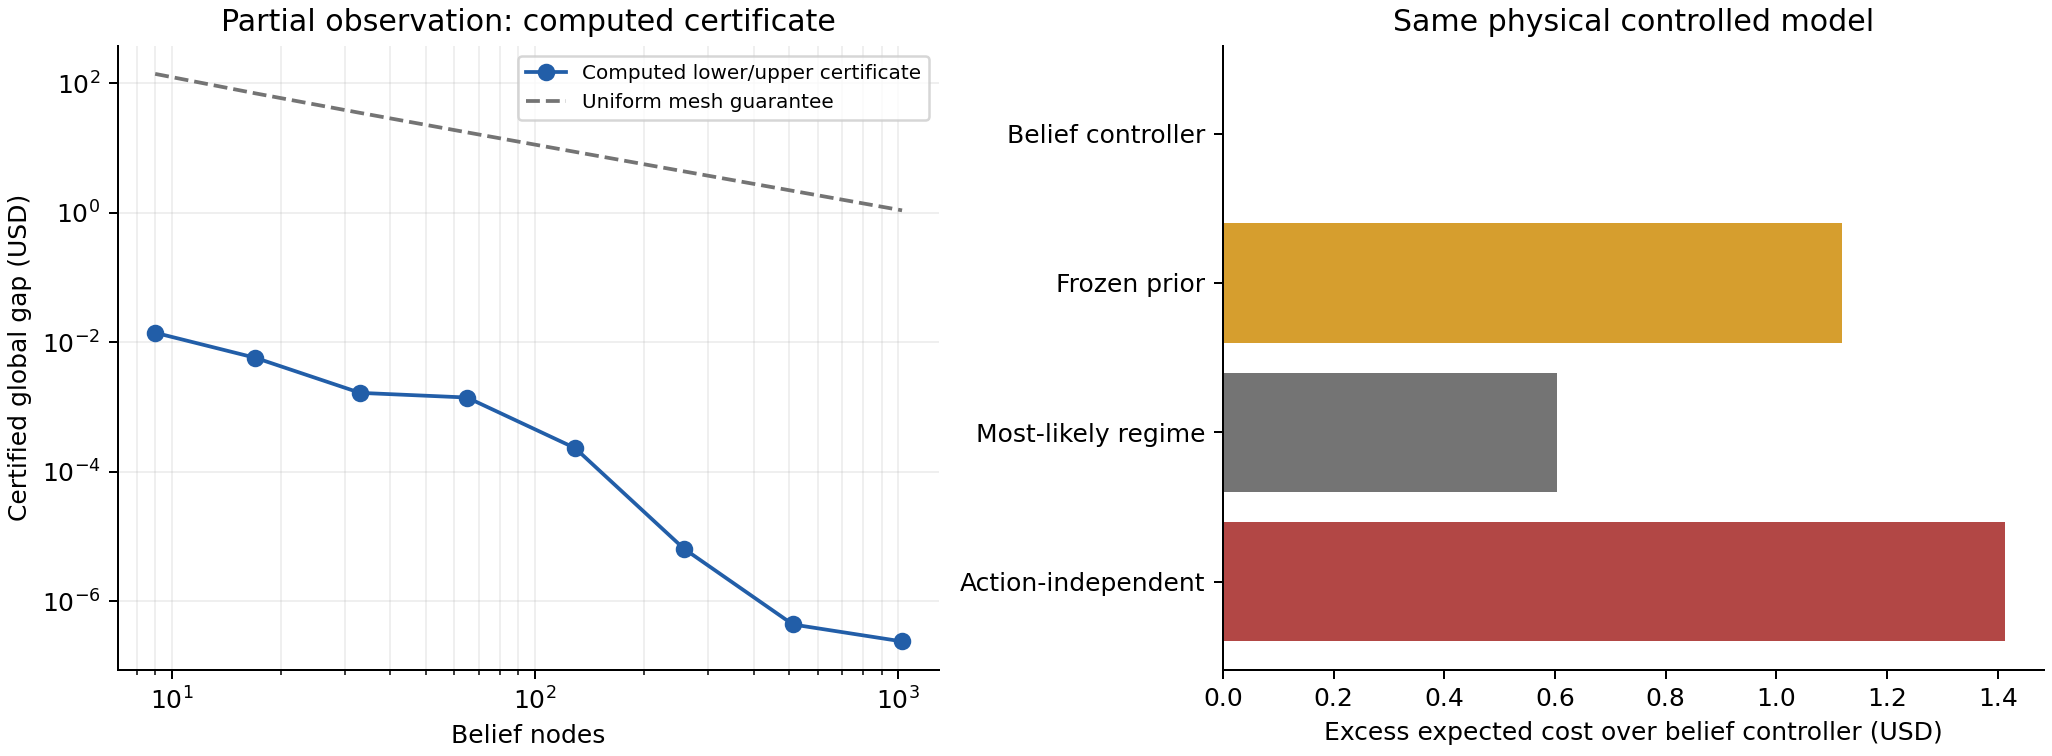
\includegraphics[width=\textwidth]{figures/10_partial_observation_certificate.png}
\caption{Computed global planning certificates and comparisons in the same
controlled hidden-liquidity model. The uniform mesh bound is deliberately
conservative. The right panel compares physically evaluated expected costs;
no hidden-state observation is supplied to these four controllers.}
\label{fig:partialcertificate}
\end{figure}

\subsubsection*{Decision comparisons and finite signature implementation}

The frozen-prior baseline solves a finite dynamic program which resets its
belief to the initial prior after each report, while retaining $T_a$ in
each one-step prediction. It is then evaluated under the persistent physical
regime. The most-likely-regime baseline filters the reports and applies the
fully observed Bellman action for the more probable regime, with a fixed
tie rule. The action-independent-transition baseline plans and filters with
$T_a=T_{\rm wait}$ for every action, retaining the action-specific fill
probabilities, and is evaluated under the true action-dependent matrices.
All three have the same instruction set, loss and completion facility.
The first and third are explicitly specified misspecified-model baselines,
not claims to optimality over every controller that omits information.

\begin{table}[tb]
\centering\small
\caption{Physical-model policy evaluation, in USD. Costs are rounded upward;
excess costs are conservative lower bounds relative to the certified belief
controller. Baseline definitions are given in the text.}
\label{tab:partialpolicies}
\begin{tabular}{lrr}
\toprule Policy & Expected-cost upper bound & Excess-cost lower bound\\
\midrule
\inputtable{tables/partial_policy_rows.tex}
\bottomrule
\end{tabular}
\end{table}

At the stated initial condition, the belief controller lowers expected
objective by approximately \PartialFrozenPct\% relative to the frozen-prior
baseline and \PartialBlindPct\% relative to the action-independent-transition
baseline. A fully observed regime oracle has expected cost
\$\PartialOracle. Its lower cost reflects extra information and is not the
partially observed optimality benchmark used in the certificate.

The preferred-action table is then converted to the finite-score signature
controller of \cref{cor:partialsignature}. The preferred action has weight
$w$ and every other admissible action has weight one. Table~\ref{tab:partialsoft}
evaluates this randomized controller itself, including its effects on future
liquidity and beliefs. For $w=2^{20}$, its certified global gap is at most
\$\PartialSoftGap. The result therefore covers an implemented finite-score
policy rather than only a deterministic limit with infinite logits.

\begin{table}[tb]
\centering\small
\caption{The implemented finite-score signature controller, using 1,025 belief
nodes. The preferred score is $\log w$; other feasible scores are zero.
Costs and gaps are in USD and displayed upward.}
\label{tab:partialsoft}
\begin{tabular}{rrr}
\toprule Preferred weight $w$ & Expected-cost upper bound & Certified global gap\\
\midrule
\inputtable{tables/partial_softmax_rows.tex}
\bottomrule
\end{tabular}
\end{table}

\begin{figure}[tb]
\centering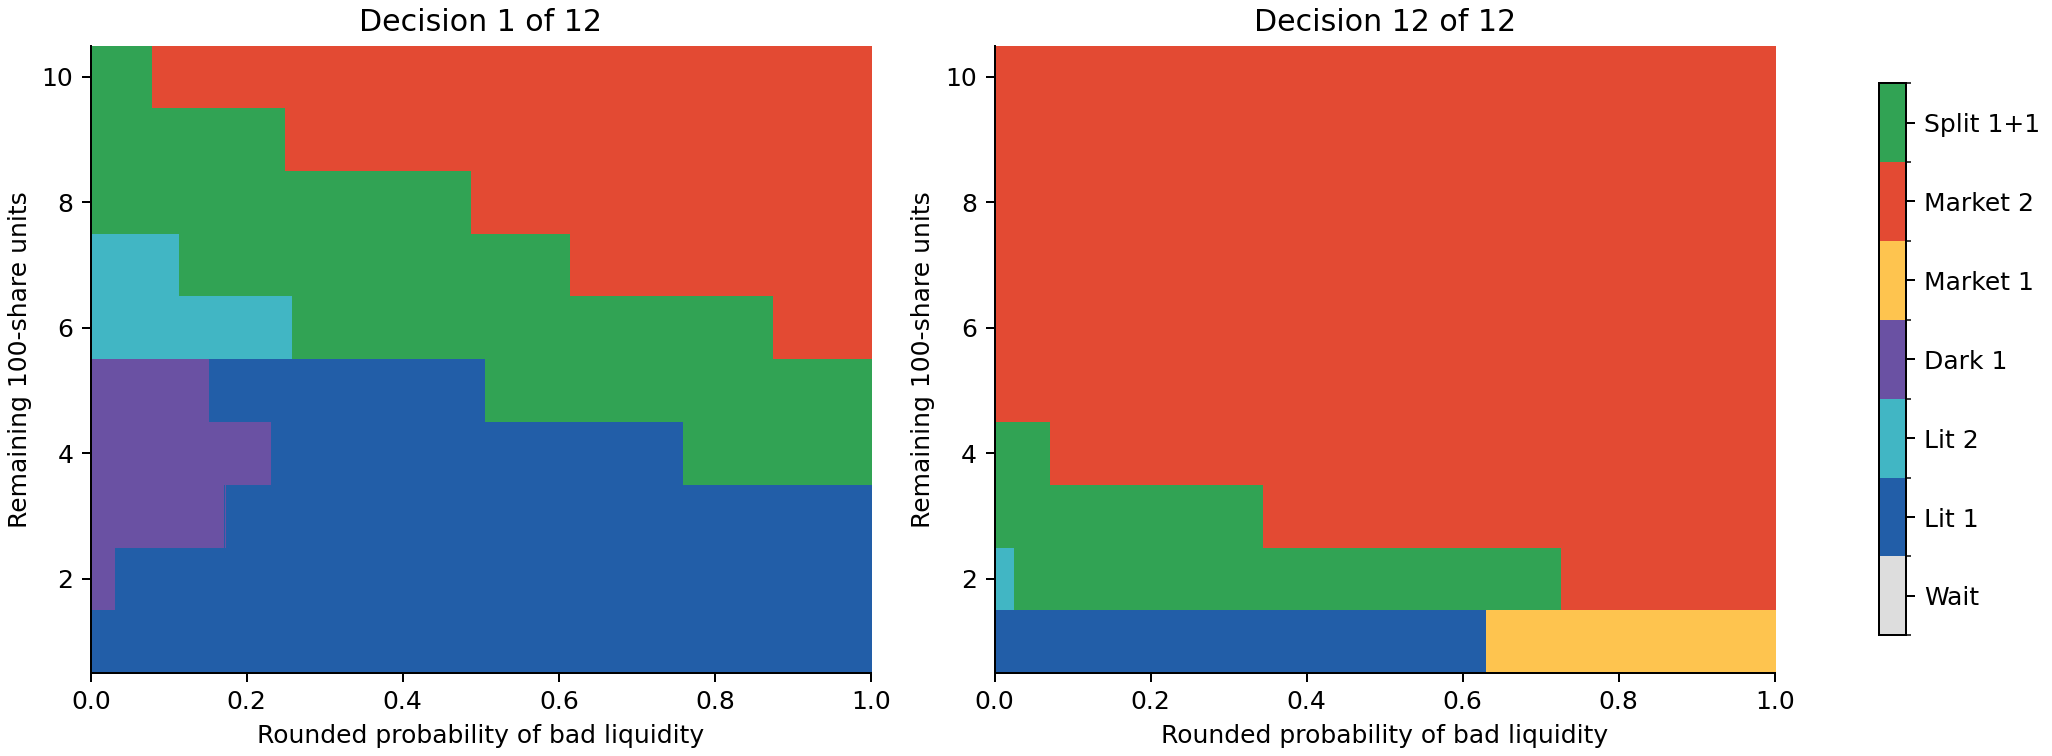
\includegraphics[width=\textwidth]{figures/11_partial_observation_policy.png}
\caption{Preferred instructions at the first and last decisions as a function
of remaining quantity and observable rounded belief. The hidden regime is
not an input. The policy table is encoded by the endpoint of the finite
observable summary channel.}
\label{fig:partialpolicy}
\end{figure}

\subsubsection*{Sensitivity and independent verification}

The same fixed economic parameters are also tested with six or twelve
decisions and initial bad-state probabilities $1/4,1/2,3/4$, using 257 belief
nodes. Table~\ref{tab:partialrobust} reports all six combinations. The belief
controller improves on both specified baselines in every case, although
the benefit varies substantially with prior and deadline. This is a
sensitivity check of the declared model, not evidence of universal superiority.

\begin{table}[tb]
\centering\small
\caption{Prior and deadline sensitivity. All USD columns use outward rounding.
The last two columns give lower bounds on baseline excess cost over the
certified controller. Every row uses 257 belief nodes.}
\label{tab:partialrobust}
\begin{tabular}{rrrrrr}
\toprule $K$ & $b_0$ & Controller cost & Global gap & Frozen-prior excess & Transition-blind excess\\
\midrule
\inputtable{tables/partial_robustness_rows.tex}
\bottomrule
\end{tabular}
\end{table}

All primitive probabilities in \eqref{eq:partialexperimentkernel} are integer
multiples of $10^{-8}$. For grid beliefs, posterior numerators and
nearest-node decisions are computed with integer arithmetic, including
ties. Elementary nonnegative products, sums and divisions in the bound
recursions are enclosed by outward expansion using the adjacent binary64
floating-point numbers. The value enclosures are approximately
$1.2\times10^{-13}$ USD wide; the global finite-grid optimization tolerance
from \eqref{eq:partialnumericalgap} is below $1.2\times10^{-12}$ USD.
The reported policy-approximation gaps are separate from these numerical
enclosure widths.

An independent exact-rational exhaustive recursion for three decisions and
two units gives
\[
 V^*=\frac{232172138011}{156250000000}=1.4859016832704.
\]
Its 3,553 distinct recursion states give a value between the grid lower bound
and the controller upper bound. Exact-rational evaluation of the deterministic
and finite-score controllers is also contained in the corresponding outward
intervals. A separate forward occupancy calculation agrees with the main
backward physical evaluation to better than $10^{-10}$ USD, conserves total
probability to better than $10^{-12}$, and visits 9,390 positive-probability
stage/memory states. The code checks 24,600 integer posterior-rounding and
probability-enclosure cases on the finest grid.

These computations are reproducible without an optimization oracle or a
Monte Carlo stopping criterion. They certify global planning accuracy for
the stated finite-observation model. Transfer to an estimated market model
still requires a justified $B_T$ in \eqref{eq:partialtransfer}; increasing
belief resolution cannot compensate for incorrect transition, reporting or
cost assumptions.
